% ==========================================================================================
\section{Exposure after Security Advisories}
\label{sec:exposure}

\subsection{Advisories gossip can see}
We collected every public security advisory for LND, CLN, Eclair and LDK from January~2022 to the cutoff (release
notes, Lightning Labs' advisory index, Delving Bitcoin and authors' write-ups), recording the affected versions, the
first fixed release and the disclosure date. An advisory is visible in gossip when its fix boundary coincides with
the start of a release line (LINE), or falls inside a line but leaves whole lines affected or fixed on either side
(PARTIAL, which gives bounds). Fixes inside the newest line, such as CLN 26.06.7--26.06.9 and Eclair 0.14.1--0.14.3,
are patch releases and invisible. Eclair and LDK have too few live public nodes with a known line (about ten Eclair
nodes) for shares to be meaningful, so Table~\ref{tab:advisories} lists the \NAdvRows{} LND and CLN entries,
covering \NAdvTotal{} advisories.

Two clocks run for each advisory. Fixes usually ship long before the vulnerability is disclosed: the median gap
between the first fixed release and disclosure is \FixToDiscMedian{} days, and the six advisories Lightning Labs
published on 11~August~2026 concerned bugs fixed in LND 0.19.0, released \FixToDiscLLBatch{} days earlier. A node
still on an affected line at disclosure has therefore usually skipped a release that was already available for many
months. Exposure is the share of live nodes (excluding the managed fleet) on an affected line, with the share of
their live capacity alongside.

\begin{table*}[t]
\centering\footnotesize
\caption{Advisories whose fix boundary is visible in gossip (LND and CLN). Exposure = share of live nodes of that implementation whose inferred release line is affected, in \%; share of their live capacity in parentheses; for PARTIAL rows (the fix lands inside a line) the bounds are given in brackets at disclosure. Fix$\to$disc.\ = days from the first fixed release to public disclosure. \# = advisories grouped in the row.}
\label{tab:advisories}
\resizebox{\textwidth}{!}{%
\begin{tabular}{lllrlrrrrr}
\toprule
Impl. & Advisory & Class & \# & Fixed in & Fix$\to$disc. & At fix & At disclosure & +60\,d & Cutoff \\
\midrule
CLN & Fake channel DoS (2023-08-23) & PARTIAL & 1 & 23.02 & 175 & -- & -- & 6 (2) & 1 (0) \\
CLN & Replacement cycling (CVE-2023-40234) (2023-10-16) & PARTIAL & 1 & 23.08.1 & 34 & -- & 38 [24--100] (17) & 26 (10) & 2 (0) \\
CLN & BOLT11 parsing bugs, batch 1 (2023-12-08) & PARTIAL & 1 & 23.02 & 282 & -- & 4 [4--95] (2) & 2 (1) & 1 (0) \\
CLN & BOLT11 parsing bugs, batch 2 (2023-12-08) & LINE & 1 & 23.11 & 10 & 99 (100) & 96 (96) & 69 (73) & 3 (0) \\
CLN & funding\_created assertion DoS (2026-05-16) & LINE & 1 & 25.09 & 256 & 98 (97) & 29 (24) & 24 (21) & 12 (2) \\
CLN & connectd queue memory exhaustion (2026-07-19) & LINE & 1 & 25.09 & 320 & 98 (97) & 24 (20) & 14 (3) & 12 (2) \\
CLN & gossipd unknown-SCID memory exhaustion (2026-07-19) & LINE & 1 & 26.04 & 90 & 100 (100) & 67 (58) & 29 (16) & 24 (13) \\
CLN & Ping-flood OOM (2026-08-25) & LINE & 1 & 25.09 & 357 & 98 (97) & 19 (16) & -- & 12 (2) \\
LND & Fake channel DoS (2023-08-23) & PARTIAL & 1 & 0.16.0 & 147 & -- & -- & 0 (0) & 1 (0) \\
LND & Replacement cycling (CVE-2023-40233) (2023-10-16) & PARTIAL & 1 & 0.17.0 & 13 & -- & 0 [0--100] (0) & 0 (0) & 1 (0) \\
LND & Premature channel\_update OOM (2023-12-21) & LINE & 1 & 0.14.0 & 764 & -- & 0 (0) & 0 (0) & 1 (0) \\
LND & channel\_update signature after rate limit (2023-12-21) & PARTIAL & 1 & 0.15.0 & 546 & -- & 0 [0--0] (0) & 0 (0) & 1 (0) \\
LND & Onion bomb (CVE-2024-38359) (2024-06-18) & PARTIAL & 1 & 0.17.0 & 259 & -- & -- & -- & 1 (0) \\
LND & Irrevocable fees / update\_fee breach fee-burn (2024-12-10) & PARTIAL & 1 & 0.18.3 & 89 & 44 (35) & 33 [33--100] (25) & 24 (11) & 4 (0) \\
LND & Excessive HTLC failback (2025-03-04) & LINE & 1 & 0.18.0 & 278 & -- & 20 (8) & -- & 4 (0) \\
LND & gossip\_timestamp\_filter goroutine DoS (2025-07-22) & PARTIAL & 1 & 0.18.3 & 313 & 44 (35) & 11 [11--60] (3) & 9 (2) & 4 (0) \\
LND & Replacement stalling, failback \#2, infinite inbox (2025-12-04) & LINE & 3 & 0.19.0 & 196 & 98 (96) & 28 (12) & 22 (10) & 13 (6) \\
LND & Zero-timestamp gossip panic (2026-06-18) & PARTIAL & 1 & 0.20.1 & 126 & 48 (73) & 34 [34--97] (27) & 25 (16) & 20 (10) \\
LND & Lightning Labs batch: gossip, peer and queue DoS (2026-08-11) & LINE & 6 & 0.19.0 & 446 & 98 (96) & 15 (6) & 13 (6) & 13 (6) \\
LND & HTLC first-stage sweep budget failure (2026-08-11) & LINE & 1 & 0.19.0 & 446 & 84 (92) & 10 (5) & 8 (6) & 8 (6) \\
LND & Too few confirmations on cooperative close (2026-08-13) & PARTIAL & 1 & 0.20.1 & 182 & 48 (73) & 25 [25--51] (17) & 21 (10) & 20 (10) \\
LND & Gossip stall via malformed announcements (2026-09-21) & PARTIAL & 1 & 0.20.1 & 221 & 27 (64) & 8 [8--32] (5) & -- & 8 (4) \\
LND & Brontide write-allocation OOM (2026-09-21) & LINE & 1 & 0.20.0 & 305 & 99 (99) & 22 (11) & -- & 20 (10) \\
\bottomrule
\end{tabular}}
\par\vspace{2pt}\parbox{\textwidth}{\footnotesize Before July 2024 our view did not include the few live nodes on LND releases older than 0.14 (\S\ref{sec:data}); exposures to the 2023 LND advisories at disclosure are lower bounds. --: no usable snapshot within 7 days.}
\end{table*}


\subsection{Disclosure barely moves LND operators}
On the day Lightning Labs disclosed its batch, \ExpLLBatchDisc\% of live LND nodes, holding \ExpCapLLBatchDisc\% of
live LND capacity, were on a line older than 0.19 (Fig.~\ref{fig:cases}). Of the \CohortLLBatch{} exposed nodes,
\CohortUpLLBatch{} had upgraded by the cutoff, \CohortLeftLLBatch{} were no longer live and \CohortStillLLBatch{}
(\PctCohortStillLLBatch\%) were still live on an affected line. The disclosure did not change the pace: in the 30 days
before it, \RateLLBatchBefore\% of the live nodes then on affected lines moved to a fixed line; in the 30 days after,
\RateLLBatchAfter\%. Morehouse's disclosure of three LND vulnerabilities fixed in the same release, on 4~December~2025,
looks the same: \ExpLndSweeperDisc\% of live LND nodes exposed, an upgrade rate of \RateLndSweeperBefore\% before and
\RateLndSweeperAfter\% after, and \PctCohortStillLndSweeper\% of the exposed cohort still exposed four months later.
The exposed nodes are small: their share of capacity is about half their share of nodes.

\subsection{CLN operators responded}
CLN's two memory-exhaustion vulnerabilities, disclosed on 19~July~2026, were fixed at the 25.09 and 26.04 line
starts. Here the disclosure changed behaviour. Among live CLN nodes on lines before 26.04, the 30-day upgrade rate
rose from \RateClnGossipdBefore\% before to \RateClnGossipdAfter\% after the disclosure (\RateClnConnectdBefore\% to
\RateClnConnectdAfter\% for lines before 25.09), and exposure kept falling after the maintainers' call on
26~August to upgrade or restart with \texttt{--offline}. Of \CohortClnGossipd{} CLN nodes exposed to the gossipd
vulnerability at disclosure, \CohortUpClnGossipd{} had upgraded by the cutoff and \CohortLeftClnGossipd{} were no
longer live, leaving \CohortStillClnGossipd{}; exposure fell from \ExpClnGossipdDisc\% of live CLN nodes to
\ExpClnGossipdCutoff\% (from \ExpCapClnGossipdDisc\% to \ExpCapClnGossipdCutoff\% of capacity). Part of the fall is
nodes leaving rather than upgrading, as in the shutdown we measured earlier~\cite{kumar2026clientdiversity}.

\begin{figure*}[t]
\centering
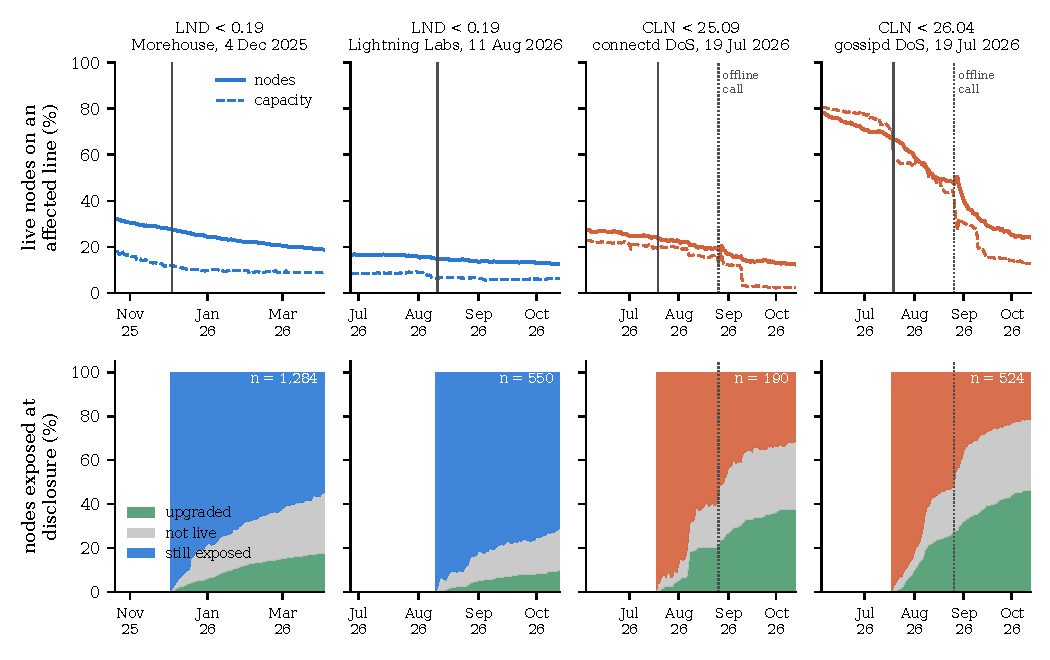
\includegraphics[width=\textwidth]{figures/fig6_exposure_cases.pdf}
\caption{Top: share of live nodes (solid) and of their live capacity (dashed) on a line affected by the advisory;
solid vertical line: disclosure; dotted: CLN's call of 26~August~2026 to upgrade or restart offline. Bottom: the nodes
exposed on the last snapshot before disclosure, by what became of them. Managed fleet excluded.}
\label{fig:cases}
\end{figure*}
